\begin{singlespacing}
\chapter{Searches in ATLAS}
\label{chapter:searches}
%
\begin{epigraphs}
\qitem{%
One way is to make it so simple that there are \emph{obviously} no deficiencies
and the other way is to make it so complicated that there are no \emph{obvious}
deficiencies.%
}%
{Tony~Hoare,
\textit{The Emperor’s Old Clothes},
1981~\cite{hoare2007emperor}}
\end{epigraphs}
\end{singlespacing}

Our task in scientific data analysis is to distil an informative
message from data and to report that message to the wider community.
From any given data there are many possible messages that could be extracted,
and those messages will have different values to different recipients of our
messages --- our data analysis is not an automatic process, but a result
of many judgements that are informed by theory, convention, and intuition.

To clarify our later description of the $\twoljets$ search in
Chapter~\ref{chapter:2ljets}, this chapter introduces the basic theory and
practice of data analysis and its manifestations in the \atlas\ SUSY community.

Theoretical data analysis in the tightly coupled fields of probability theory
and decision theory is introduced in Section~\ref{sec:searces_data_analysis}.
The attempted alternative formulation of frequentist theory is discussed in
Section~\ref{sec:searches_frequentist}.
In practice, our field of research applies modified frequentist methods to
avoid up some of their more drastic flaws; these practices are
described in Section~\ref{sec:searches_practice}.
Searches for Supersymmetric signals in \atlas\ follow a standard strategy for
their data analysis; its procedures, nomenclature, and parametric modelling
are introduced in Section~\ref{sec:searches_searches}.


\section{Data analysis}
\label{sec:searces_data_analysis}

\begin{figure}[tp]
\centering
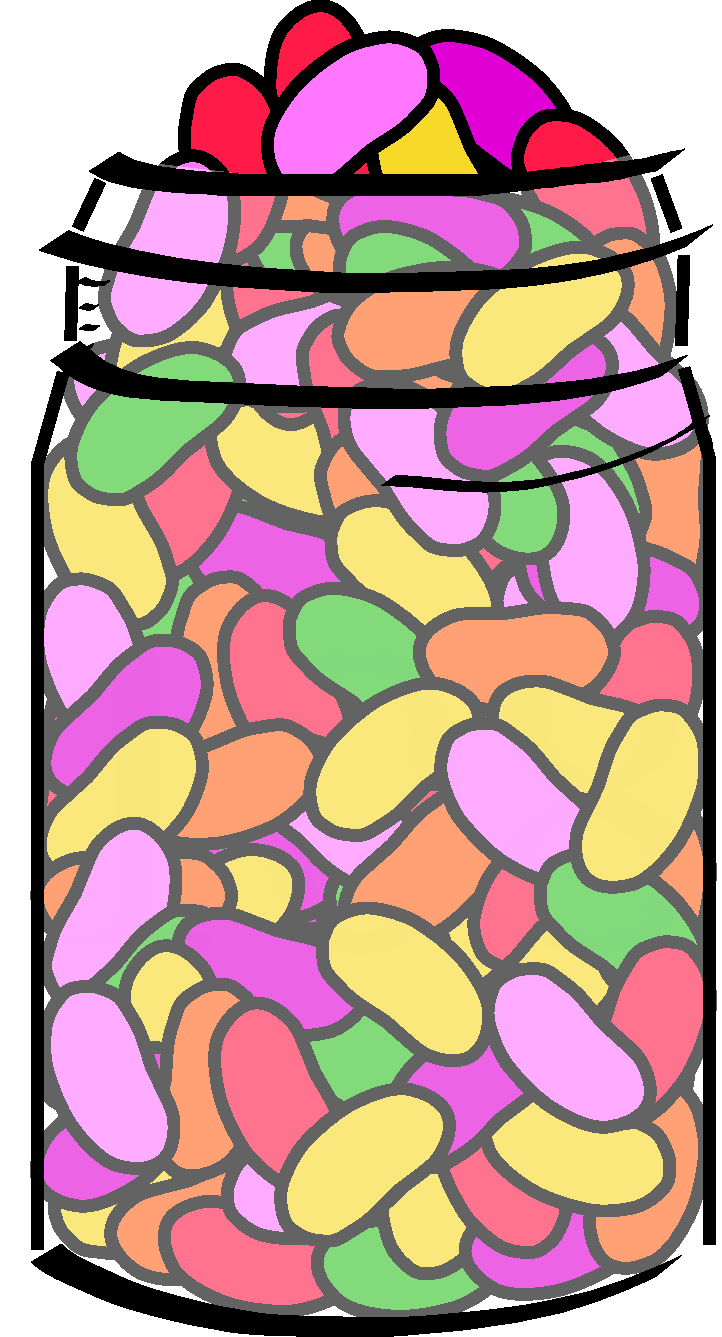
\includegraphics[width=0.25\textwidth]{figures/searches_beans.pdf}
\caption[
How many beans are in the jar?
]{%
How many beans are in the jar? This jar of jelly beans is a vehicle for our
discussion of inference and decision theory.
}
\label{fig:significant_beans}
\end{figure}

\begin{figure}[tp]
\centering
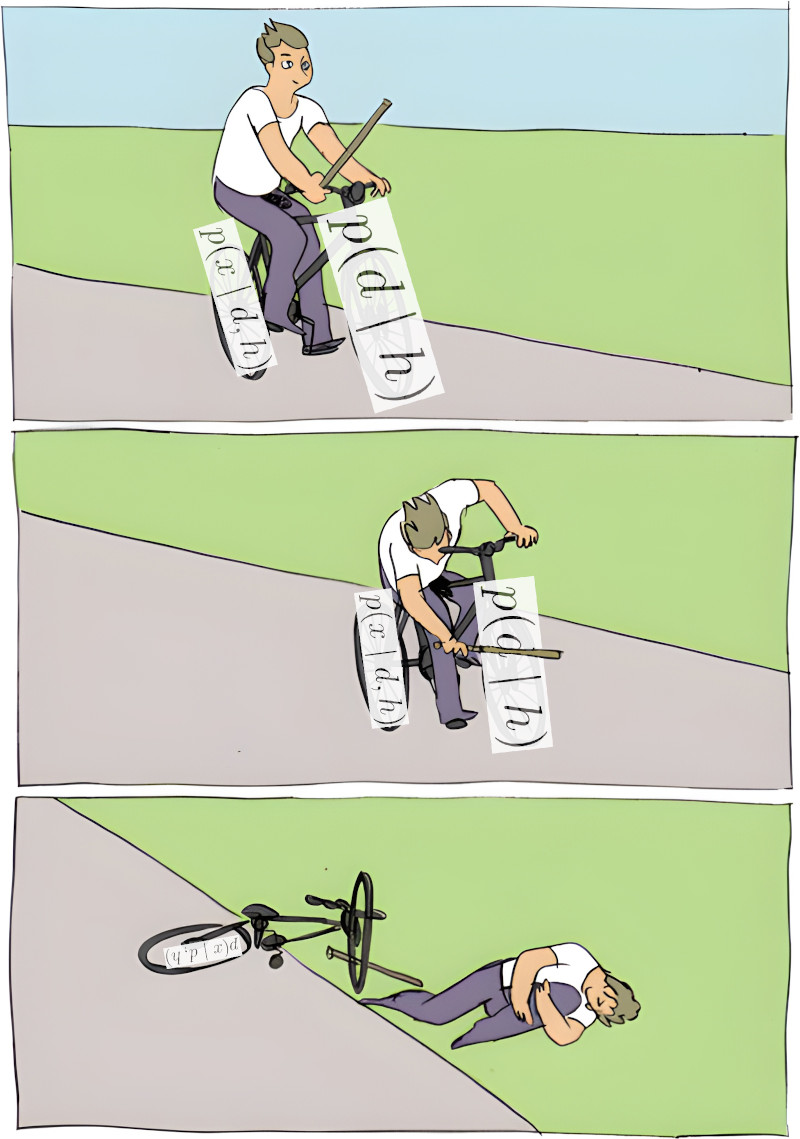
\includegraphics[width=0.6\textwidth]{figures/searches_baton_roue_bayes.jpg}
\caption[
Bayesian analysis produces two outputs: the evidence and posterior
]{%
Bayesian analysis produces two outputs: the
evidence $\prob{d}{h}$ and
posterior $\prob{x}{d,h}$ for hypothesis $h$, data $d$, and parameters $x$.
Posterior-only, semi-Bayesian methods are legitimately criticized because they
do not challenge the hypotheses that assign their priors $\prob{x}{h}$.
Since the evidence is a likelihood function over hypotheses, considering the
evidence can challenge those priors.
\\[0.5em]
Cartoon adapted from ``Baton roue'' by
Corentin~Penloup~\cite{penloup2011baton}.
}
\label{fig:searches_baton_roue_bayes}
\end{figure}

\begin{singlespacing}
\section{Frequentist theory}
\label{sec:searches_frequentist}
\begin{epigraphs}
\qitem{%
Within this theory, statistical methods of great practical usefulness have been
developed, and its statements can and frequently do contribute in a vague way
to the interpretation of data. \ldots%
}%
{John~W.~Pratt,
\textit{Review: Testing Statistical Hypotheses},
1961~\cite{pratt1961testing}}
\end{epigraphs}
\end{singlespacing}

\begin{figure}[tp]
\centering
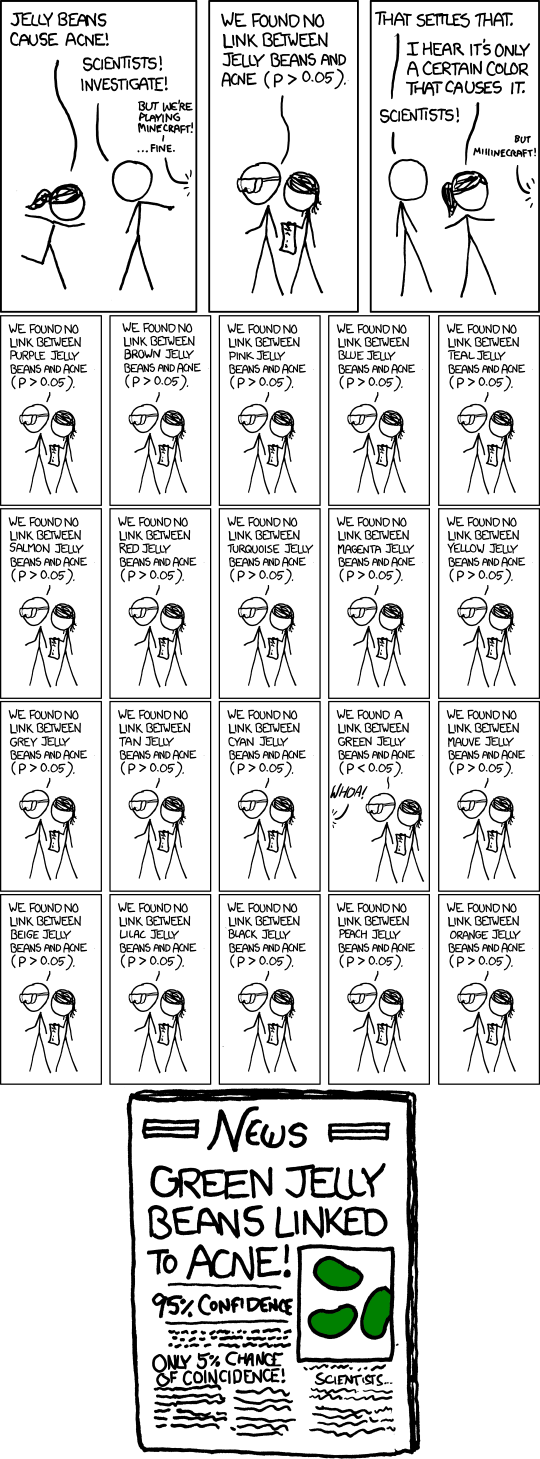
\includegraphics[width=0.55\textwidth]{figures/searches_significant_shrink.png}
\\
\begin{footnotesize}
`So, uh, we did the green study again and got no link. It was probably a{-}{-}'
\\
`RESEARCH CONFLICTED ON GREEN JELLY BEAN ACNE LINK; MORE~STUDY~RECOMMENDED!'
\end{footnotesize}
\caption[
``Significant'' by Randall~Munroe
]{%
``Significant'' by Randall~Munroe~\cite{xkcd2011significant}.
}
\label{fig:searches_significant}
\end{figure}


\begin{singlespacing}
\section{Post-frequentist practice}
\label{sec:searches_practice}
\begin{epigraphs}
\qitem{%
\ldots\ But this book, by its very excellence, its thoroughness, lucidity and
precision, intensifies my growing feeling that nevertheless the theory is
arbitrary, be it however ``objective,'' and the problems it solves, however
precisely it may solve them, are not even simplified theoretical counterparts
of the real problems to which it is applied.%
}%
{John~W.~Pratt,
\textit{Review: Testing Statistical Hypotheses},
1961~\cite{pratt1961testing}}
\end{epigraphs}
\end{singlespacing}


% significance measures
The ATLAS-recommended significance measure~\cite{atlas_significance} is
\begin{align}
\label{eqn:significance_atlas}
S_\mathrm{\atlas}(n; \mu, \sigma) =~&
\sqrt{2} \times
\mathrm{sign}(n - \mu) \times
\\[0.2em] \nonumber
&
\sqrt{
n\log\left(\frac{n(\mu + \sigma^2)}{\mu^2 + n\sigma^2}\right)
- \frac{\mu^2}{\sigma^2}\log\left(
1 + \frac{\sigma^2(n - \mu)}{\mu(\mu + \sigma^2)}
\right)
}
,
\end{align}
in an appropriate limit where $0\log(0x) = 0$ for the $n=0$ case.


\section{Searches}
\label{sec:searches_searches}
% histograms, CR VR SR, systematics
% histfactory

To model the consequences of these many factors of uncertainty, each factor is
assigned a real-valued parameter which when varied changed the expected yields
in the hisogram bins of the search.
In this way, we form a statistical model which is a function
\begin{equation}
H_{\!f}(\vec \theta) \rightarrow (\vec \mu, \log f)
\end{equation}
from the parameters $\theta$ to Poisson expectations $\vec\mu$ the histogram
bins and a regularization term $\log f$ which is maximized in fitting.

\histfactory~\cite{cranmer2012histfactory}
\pyhf~\cite{heinrich2021pyhf}
\histfitter~\cite{Besjes_2015,baak2015histfitter}


\clearpage

Hello again
